\documentclass[12pt]{article}

\usepackage{amsmath}
\usepackage{geometry}
\usepackage{setspace}
\usepackage{graphicx}
\usepackage{fancyhdr}
\usepackage{xcolor}
\usepackage{titlesec}
\usepackage{booktabs}
\usepackage{hyperref}

\hypersetup{
    colorlinks=true,       % Enable colored links
    linkcolor=blue,        % Color of internal links
    filecolor=magenta,     % Color of file links
    urlcolor=cyan          % Color of external links
}


\usepackage{url}
\geometry{a4paper, margin=1in}
\setlength{\parindent}{0pt}
\setstretch{1.5}
\usepackage{setspace}


% Header and Footer
\pagestyle{fancy}
\fancyhf{}
\fancyhead[L]{\textbf{19-AIBM4}} % Top-left text
\fancyhead[C]{\rule{\textwidth}{0.5pt}} % Top horizontal line
\fancyfoot[C]{\rule{\textwidth}{0.5pt}} % Bottom horizontal line
\fancyfoot[R]{\thepage} % Page number on the right
 

% Title formatting
\titleformat{\section}[block]
  {\large\bfseries\sffamily\color{red}}
  {\thesection.}{1em}{}

\titleformat{\subsection}[block]
  {\normalsize\bfseries\sffamily\color{red}}
  {\thesubsection}{1em}{}

\begin{document}
\pagenumbering{arabic} % Ensure Arabic numbering starts from the first page


 
% -------------------------------------------------------------
% COVER PAGE
% -------------------------------------------------------------
\begin{titlepage}
\centering
% University logo or other image

\includegraphics[width=0.4\textwidth]{UoD_Engineering.jpg} \\
\vspace{20mm}

% Title and subtitle
{\LARGE \textbf{Feasibility Report for 19-AIBM4 Autonomous Material Mover}} \\[10pt]

\vspace{5mm}\hrule\vspace{15mm}

% Insert image with caption for the material mover
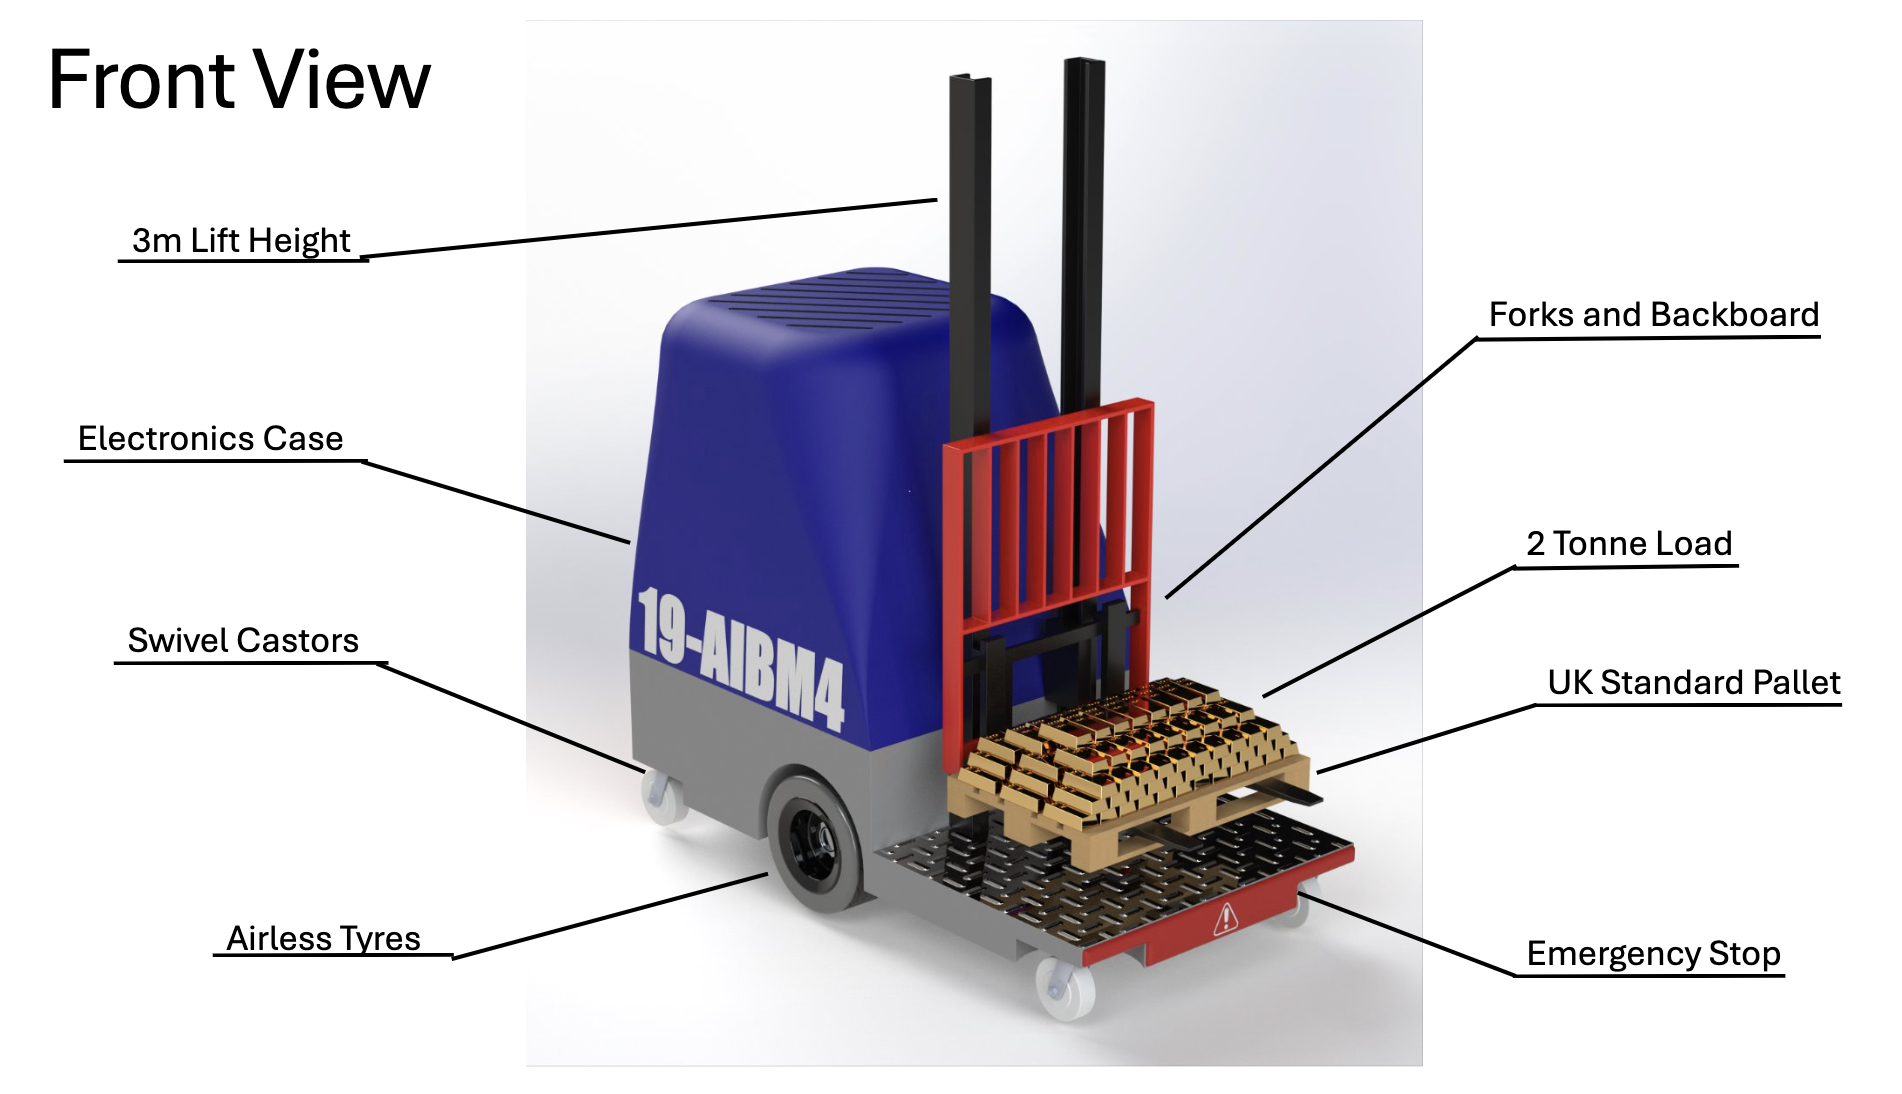
\includegraphics[width=0.8\textwidth]{Screenshot 2024-11-14 at 17.52.59.png}  \\  
\vspace{5mm}
\textit{Figure: Front View of the 19-AIBM4 Autonomous Material Mover} \\

\vspace{20mm}

% Title and author block
{\large \textbf{Co-first authors alphabetical-order}: Abi Wright, Anna Wigmore, Henry Billing, Jiaxi Wang, Louis Nangle, Will Woodward} \\ \vspace{2mm}
{Supervisor: Aissa Ikhlef, Bill Maxwell} \\[10pt]
{\small The University of Durham \\ \today}
\end{titlepage}

% -------------------------------------------------------------
% FRONTMATTER
% -------------------------------------------------------------
\tableofcontents
%\begin{figure}[h!]
 %   \centering
 %    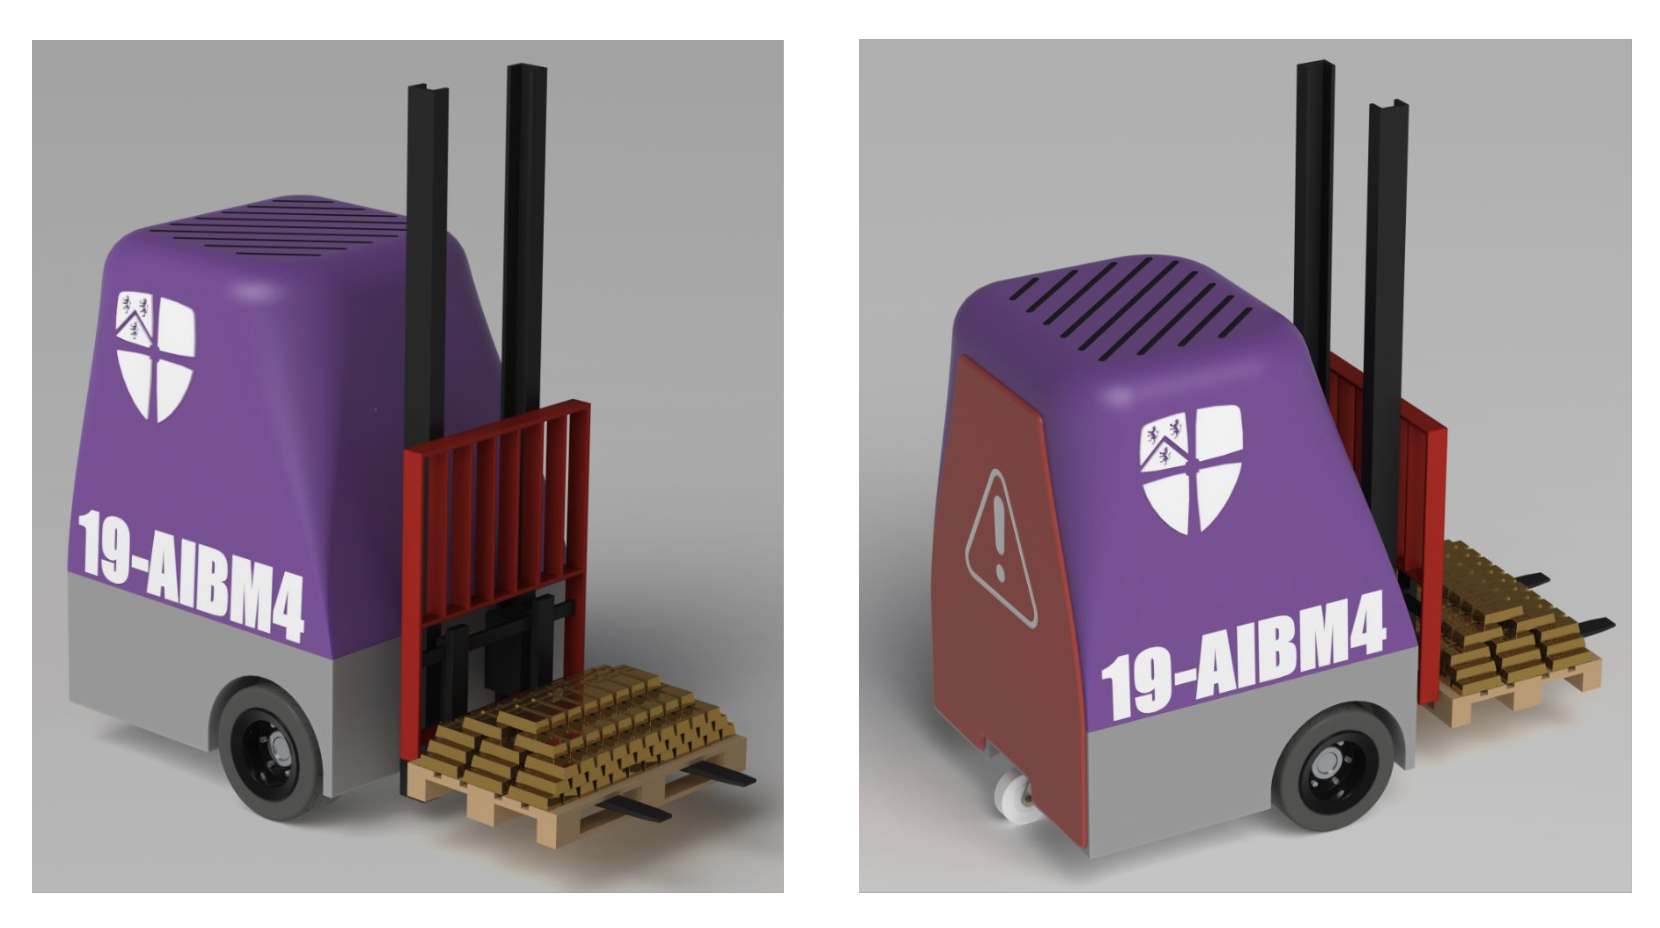
\includegraphics[width=0.65\textwidth]{finaldesign.png}
 %         \label{fig:final design}
%\end{figure}

\newpage

% -------------------------------------------------------------
% MAIN CONTENT
% -------------------------------------------------------------


% -------------------------------------------------------------
% 2. Introduction and Project Scope
% -------------------------------------------------------------
\section{Introduction}
\subsection{What is the problem that you’re attempting to solve?}
Efficient material handling is essential in modern manufacturing, but conventional forklifts still require manual operation. This project seeks to eliminate manual dependency by designing an autonomous material mover.
 
  

 

\section{Project Scope}
The estimated budget for this project is £60,000, covering labor, material mover parts, wiring, software, and programming.


\begin{figure}[h!]
    \centering
    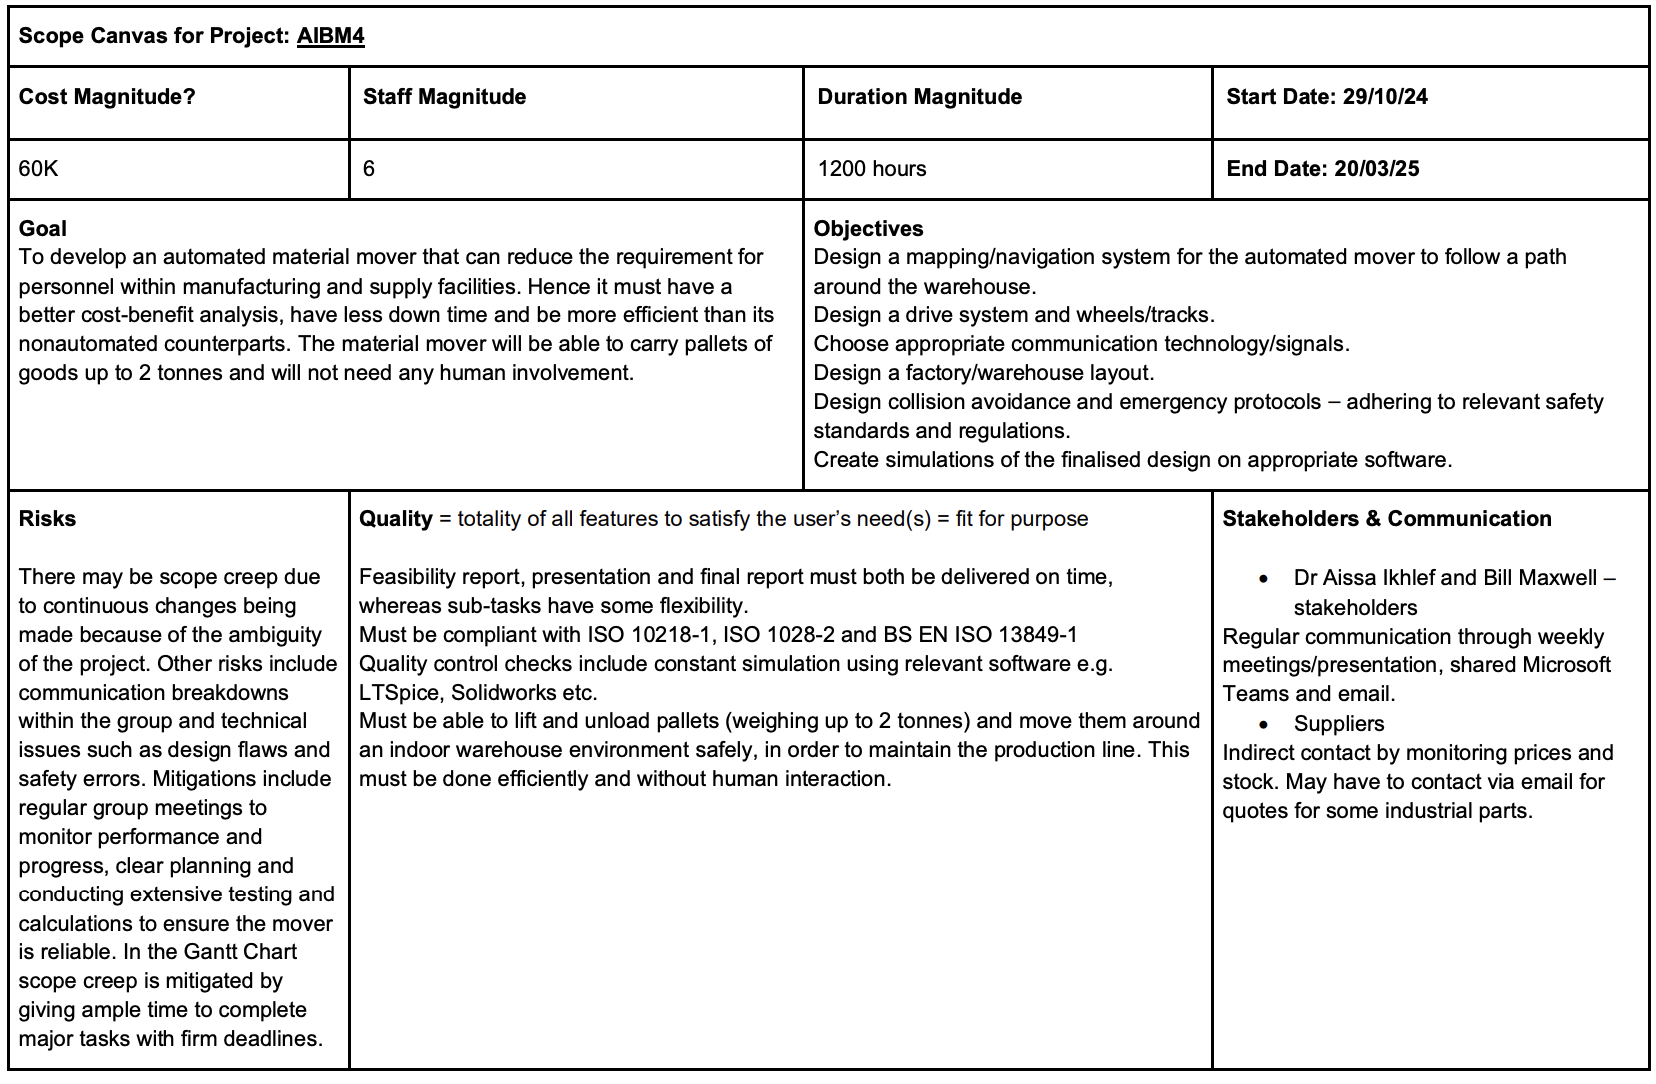
\includegraphics[width=1\textwidth]{scope1.png}
  \label{fig:Project Scope Document for AIBM4}
\end{figure}

\begin{figure}[h!]
    \centering
     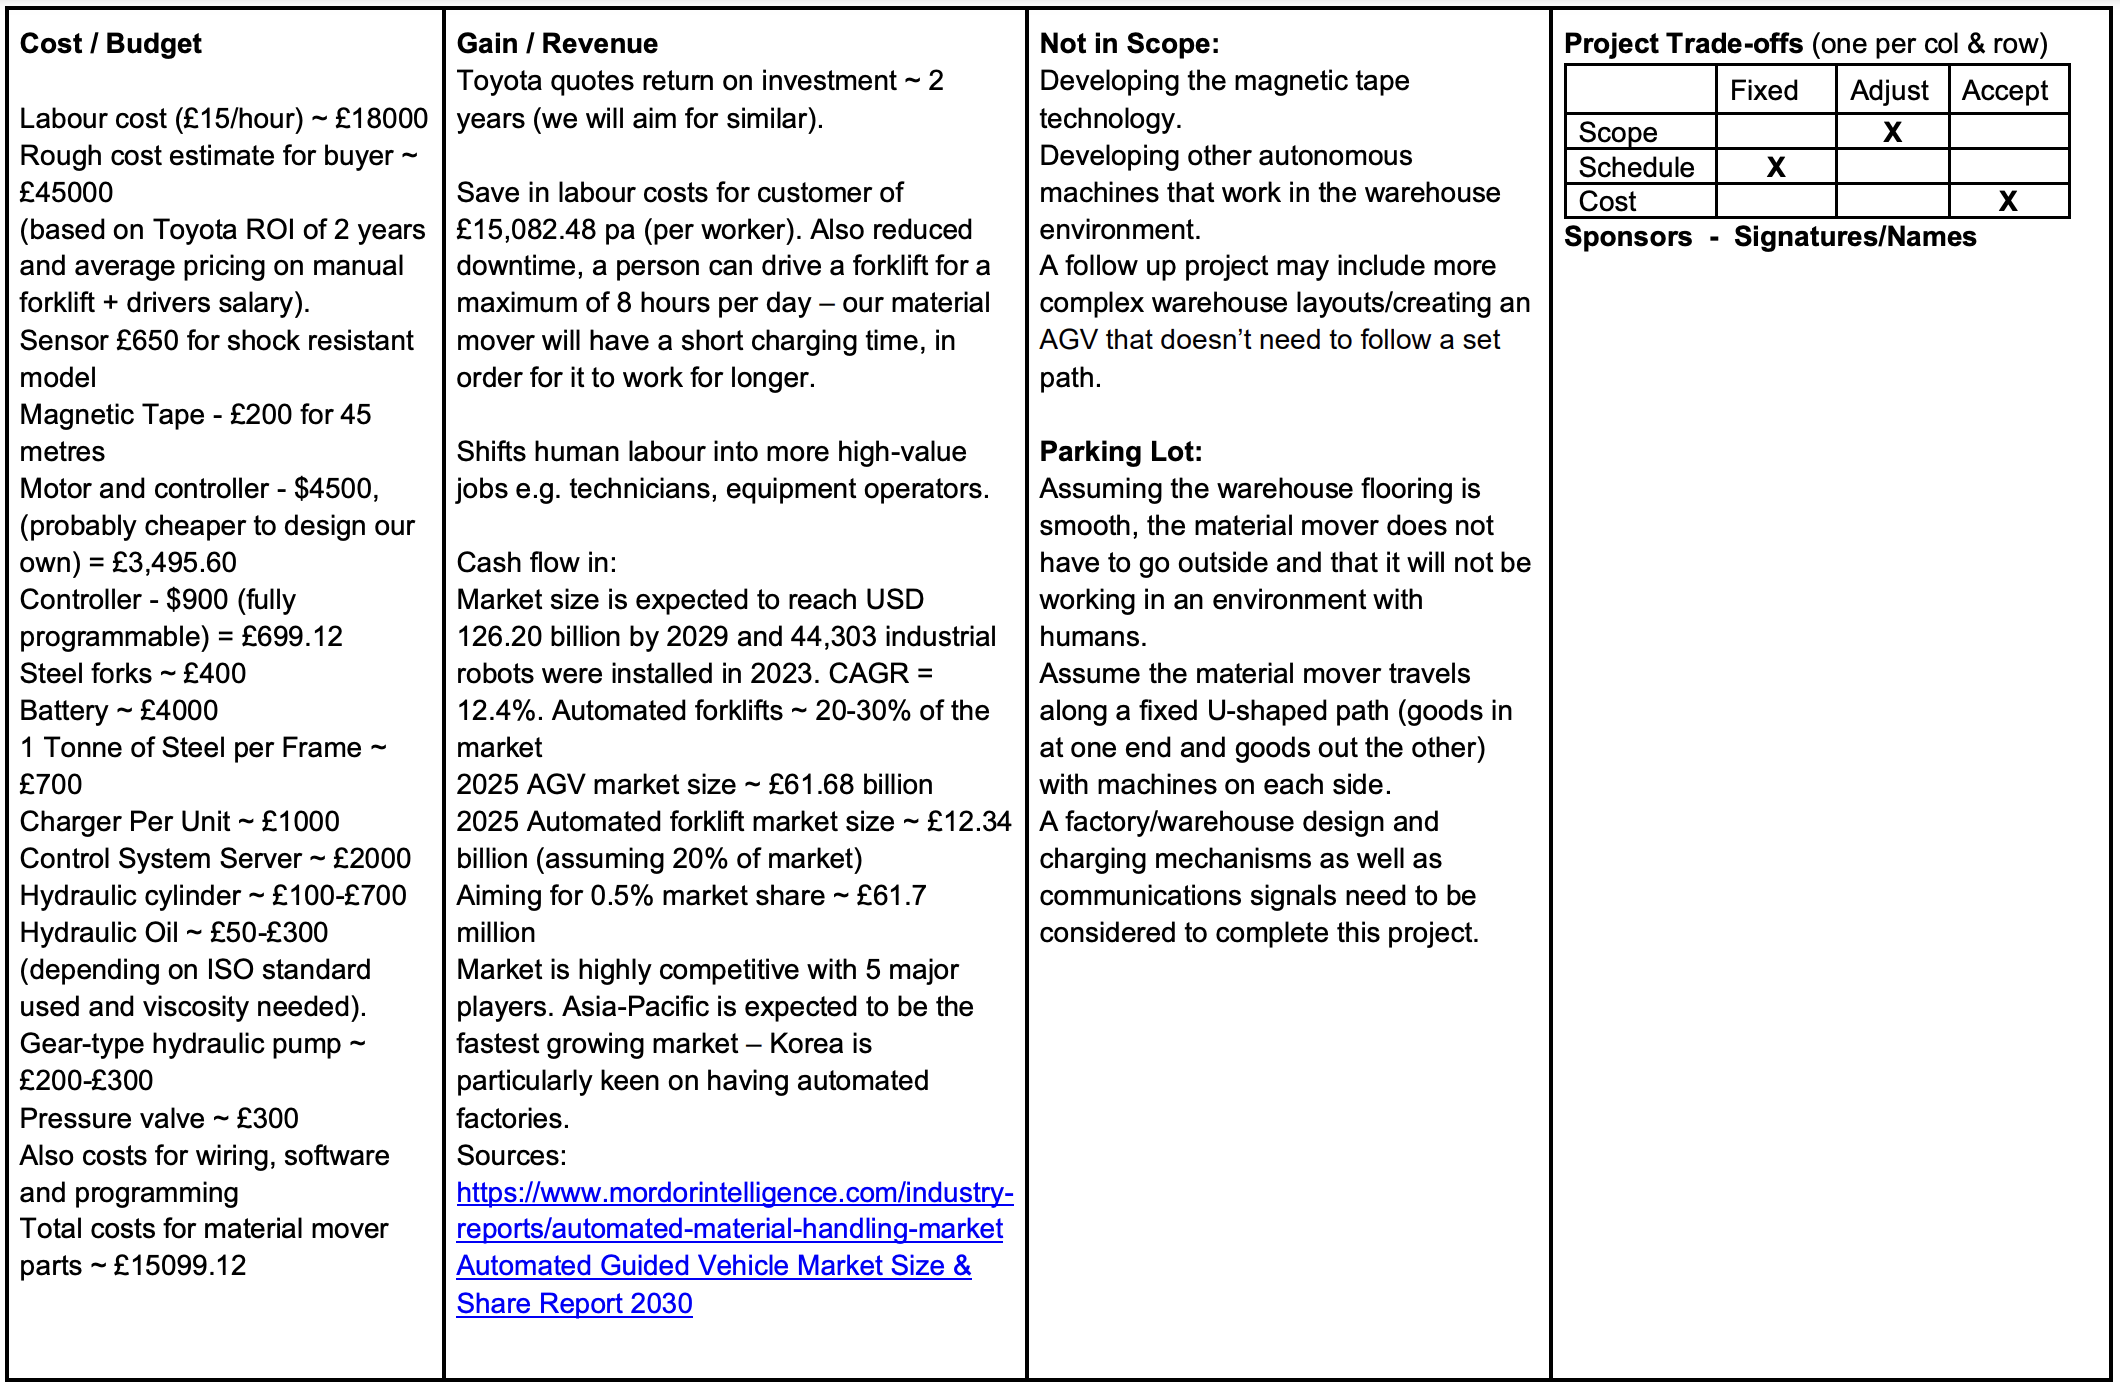
\includegraphics[width=1\textwidth]{scope2.png}
        \caption{Detailed Scope, Objectives, and Resources for Project AIBM4, focused on developing an automated material mover to enhance efficiency in manufacturing and supply facilities.}
         \label{fig:Project Scope Document for AIBM4}
\end{figure}



\newpage
% -------------------------------------------------------------
% 3. Concepts
% -------------------------------------------------------------
\section{Concepts}
\subsection{Possible Concepts}
Three design concepts were considered:
\begin{enumerate}
    \item A three-wheeled automated forklift with line-following sensors.
    \item A four-wheeled heavy-duty material mover with obstacle detection.
    \item A hybrid robotic arm integrated into a mobile platform for versatile handling.
 

 \begin{figure}[h!]
    \centering
    \begin{minipage}{0.48\textwidth}
        \centering
        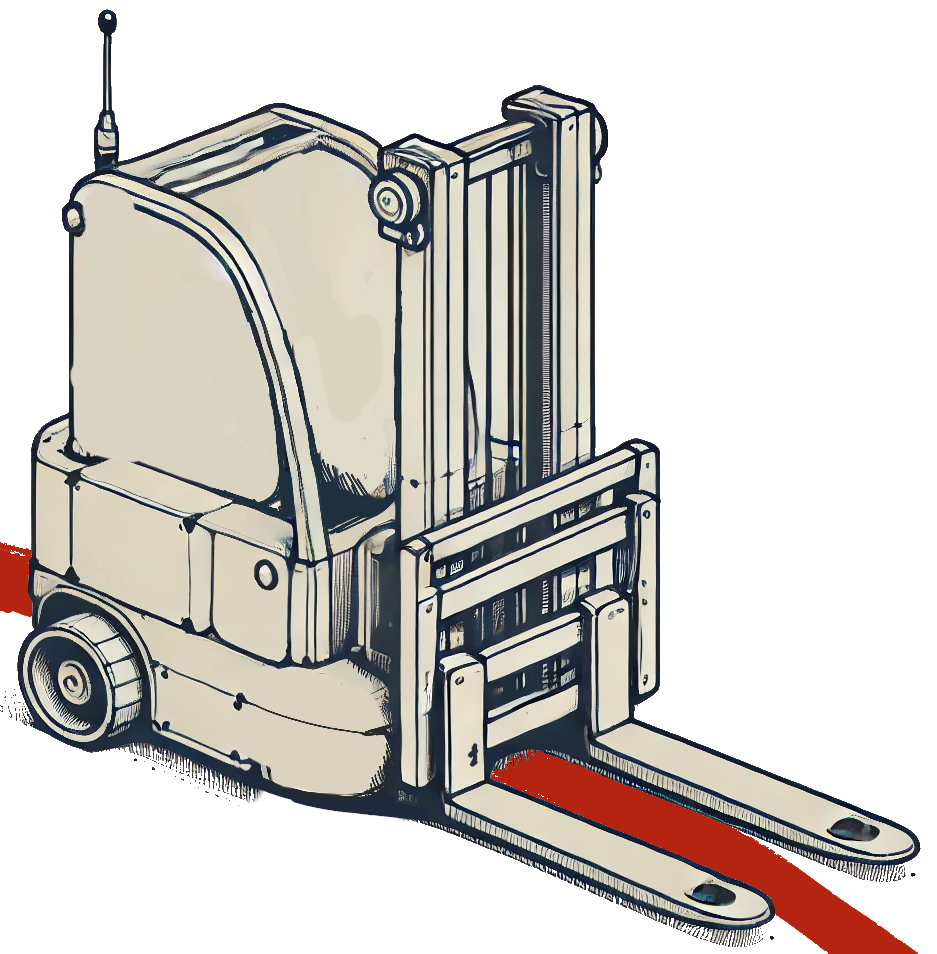
\includegraphics[width=\textwidth]{Simple_sketch_of_an_automated_forklift_robot_with_two_wheels_at_the_back_and_one_wheel_in_the_front.png}
        \caption{Jiaxi and Abi's design}
        \label{fig:three_wheel_line_flowing}
    \end{minipage}
    \hfill
    \begin{minipage}{0.48\textwidth}
        \centering
        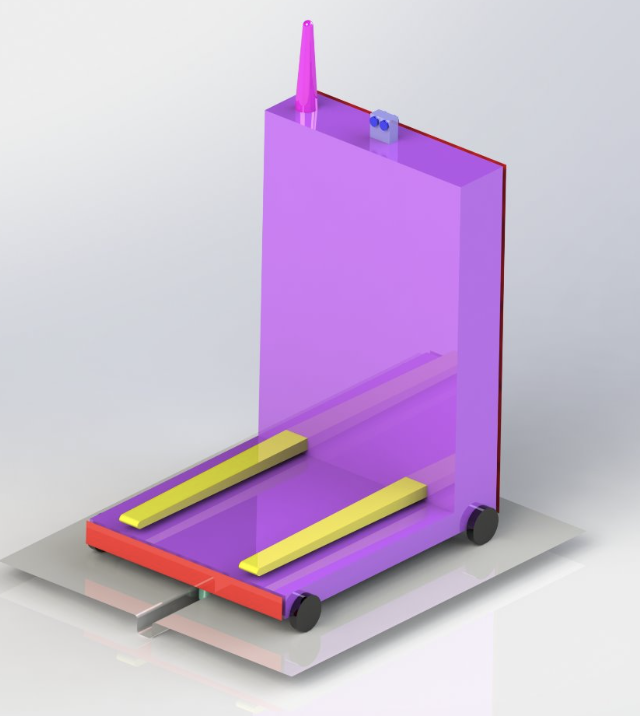
\includegraphics[width=\textwidth]{anna&will's design.png}
        \caption{Anna and Will's design idea}
        \label{fig:design_idea}
    \end{minipage}
\end{figure}

\begin{figure}[h!]
    \centering
    \begin{minipage}{0.48\textwidth}

        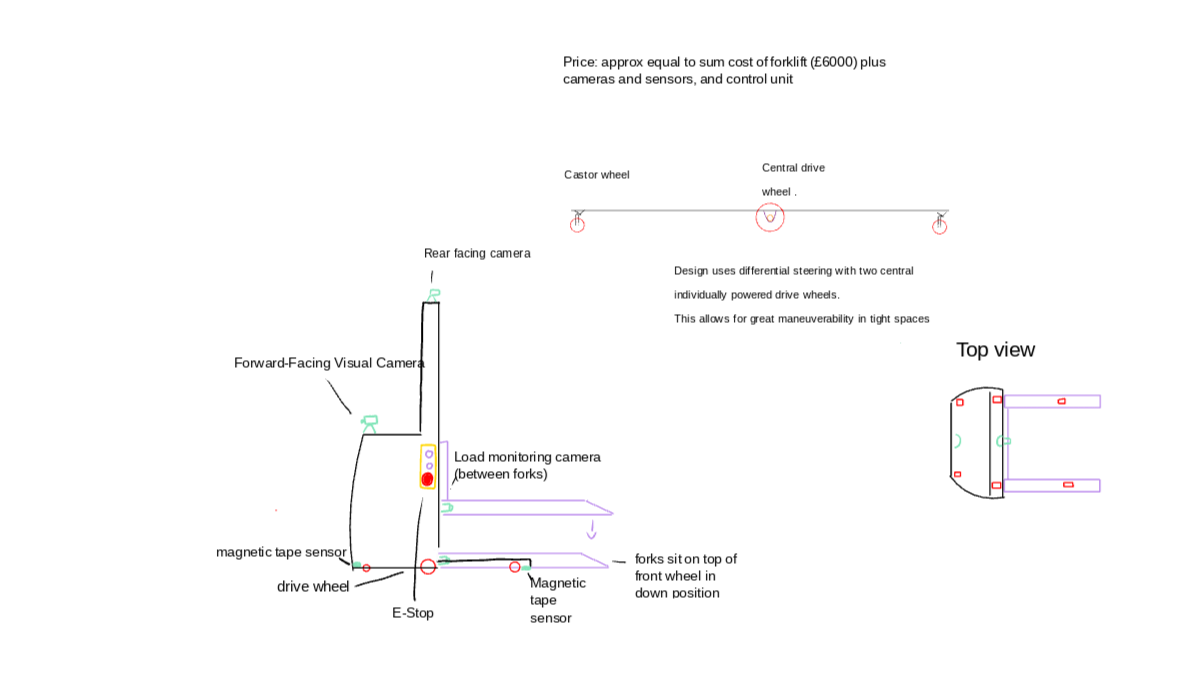
\includegraphics[width=1\textwidth]{Louis's design.png}
        \caption{Louis's design}
        \label{fig:louis_design}
    \end{minipage}
    \hfill
    \begin{minipage}{0.48\textwidth}
      
        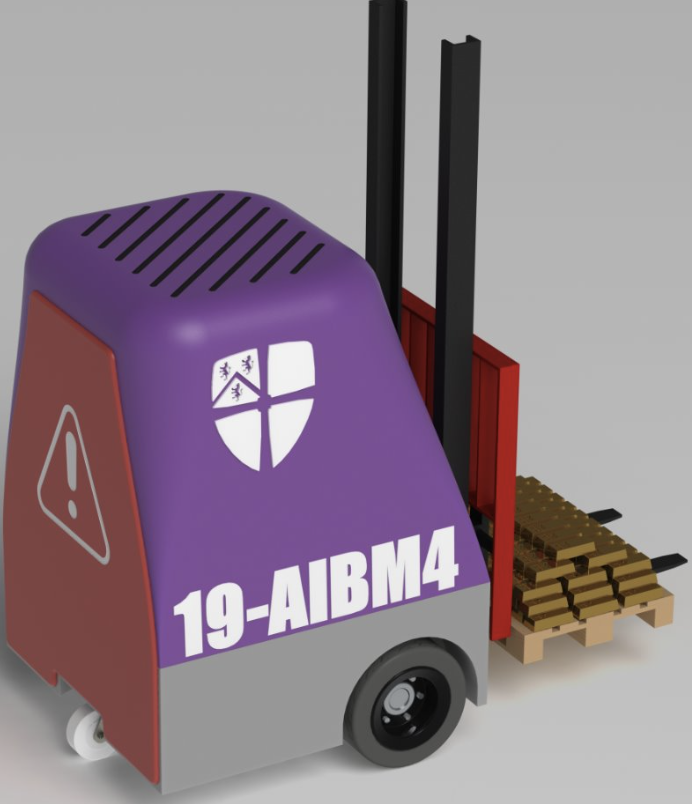
\includegraphics[width=\textwidth]{finaldesign1.png}
        \caption{Final design}
        \label{fig:final_design}
    \end{minipage}
\end{figure}


\end{enumerate}

\subsection{Strengths and Weaknesses}
Each concept was evaluated against the URS. A summary of strengths and weaknesses is provided in Table \ref{tab:concept_evaluation}.
\begin{figure}[h!]
    \centering
     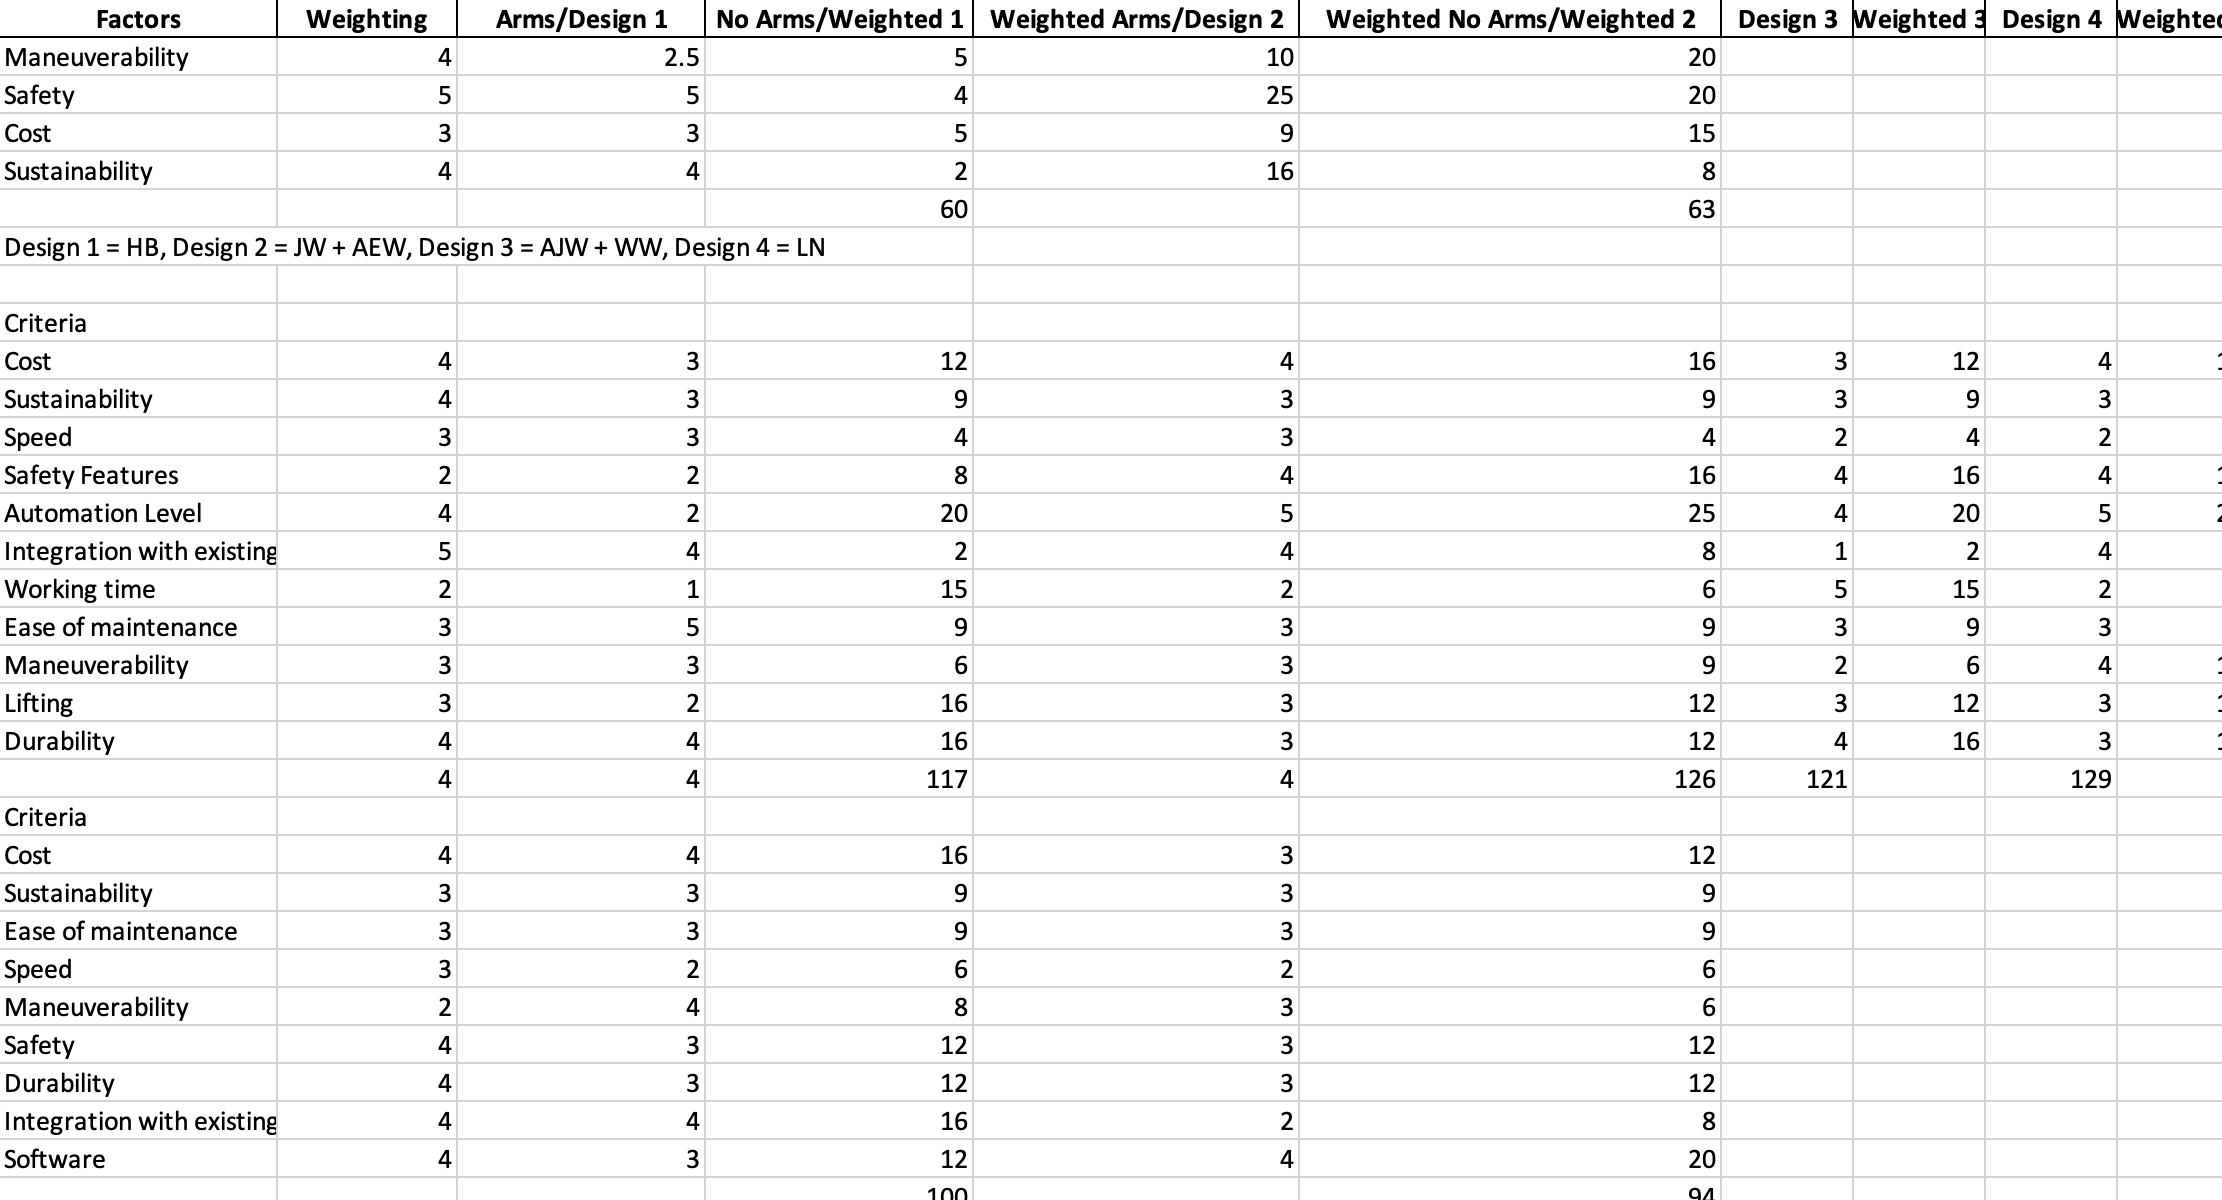
\includegraphics[width=1\textwidth]{matrix.png}
        \caption{matrix}
         \label{fig:matrix}
 
  
\end{figure}
 

\begin{table}[h!]
\centering
\caption{Concept Evaluation Matrix}
\begin{tabular}{@{}lcc@{}}
\toprule
\textbf{Criteria}      & \textbf{Concept 1} & \textbf{Concept 2} \\ \midrule
Load Capacity          & High               & Medium             \\
Navigation Efficiency  & Medium             & High               \\
Cost                   & Low                & Medium             \\
Ease of Maintenance    & High               & Low                \\ \bottomrule
\end{tabular}
\label{tab:concept_evaluation}
\end{table}

% -------------------------------------------------------------
% 4. Chosen Solution(s)
% -------------------------------------------------------------
\section{Chosen Solution(s)}

\subsection{Proposed Solution}
The three-wheeled heavy-duty material mover, is chosen due to its balance of cost, efficiency, and reliability.
\subsection{Concept Evaluation Matrix}

\subsection{Expected Cost}

 
The estimated cost of the product is £60,000, broken down as follows:


\begin{figure}[h!]
    \centering
     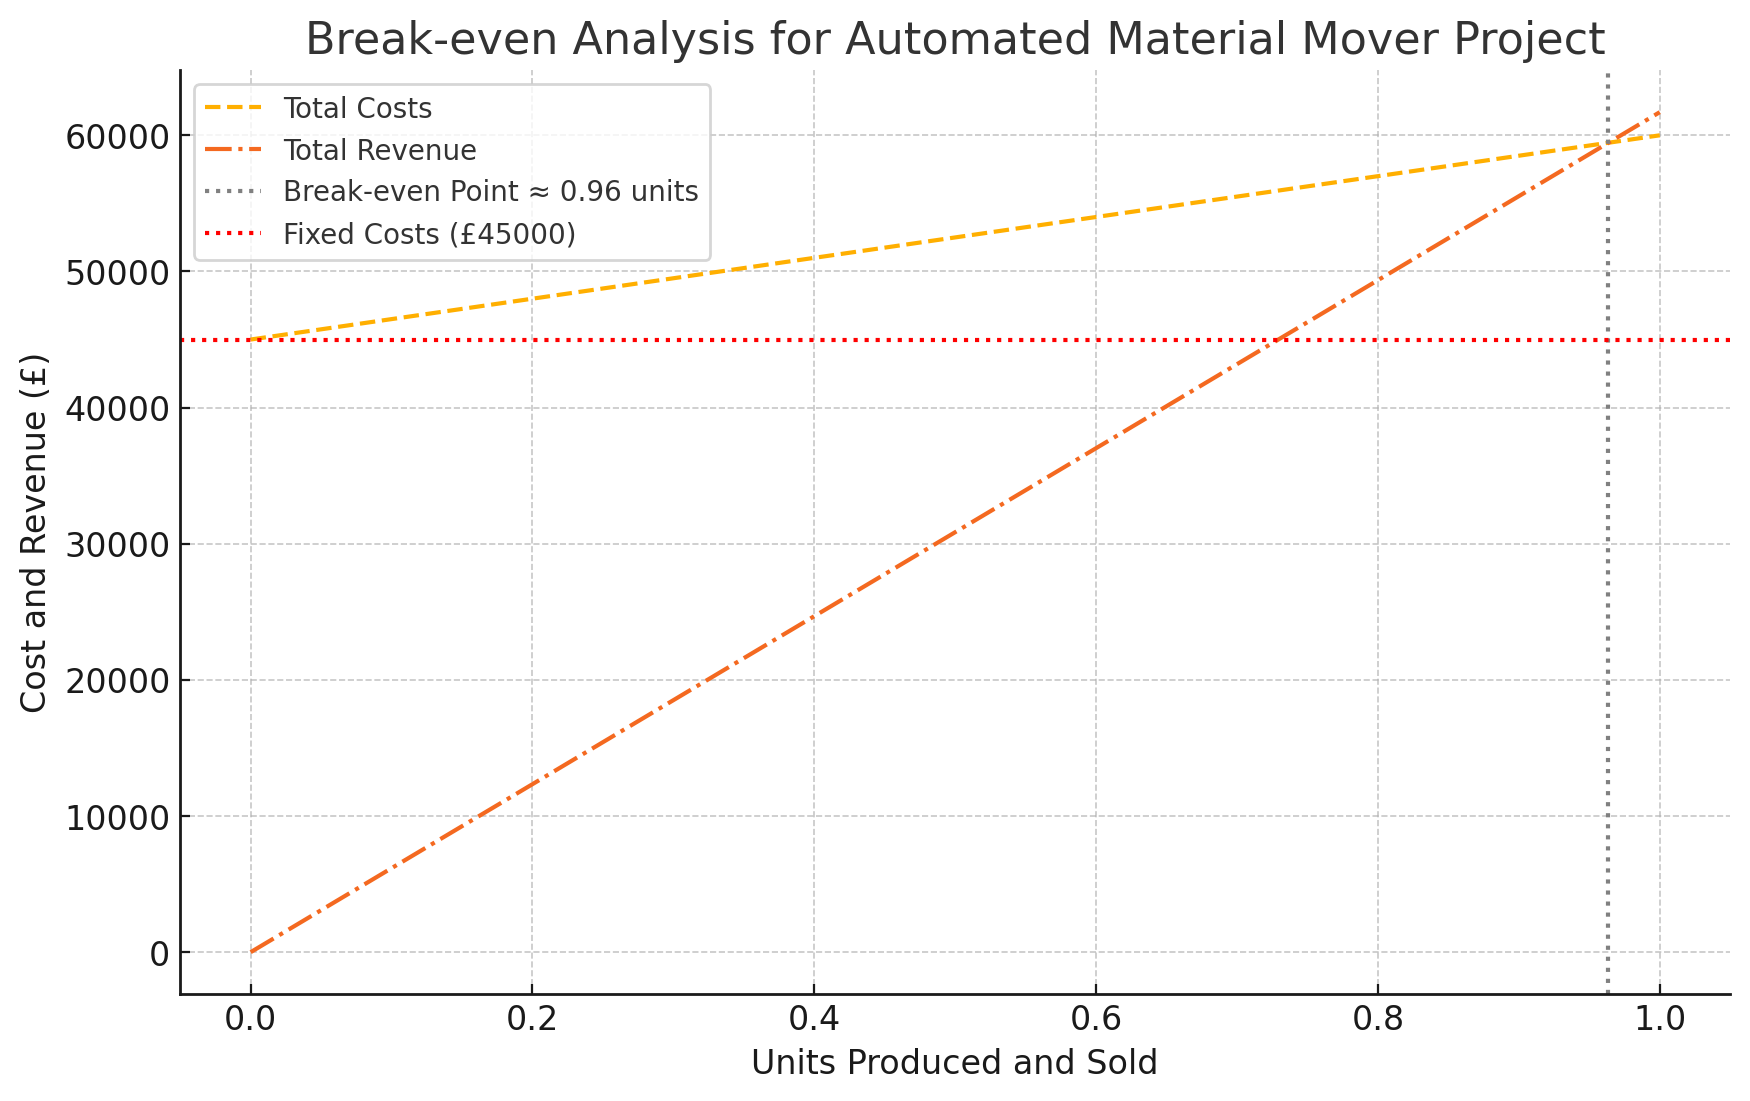
\includegraphics[width=0.6\textwidth]{breakeven.png}
        \caption{breakeven.png}
         \label{fig:timeline}
\end{figure}


\begin{table}[h!]
    \centering
    \begin{tabular}{|l|r|}
        \hline
        \textbf{Cost Item}          & \textbf{Amount (£)} \\ \hline
        Labor Costs                 & 18,000.00           \\ \hline
        Material Costs              & 15,099.12           \\ \hline
        Overheads                   & 10,000.00           \\ \hline
        Software and Simulation     & 2,000.00            \\ \hline
        Contingency                 & 4,900.88            \\ \hline
        \textbf{Total Estimated Cost} & \textbf{60,000.00}  \\ \hline
    \end{tabular}
    \caption{Breakdown of Expected Costs for the Autonomous Material Mover}
    \label{tab:expected_costs}
\end{table}


% -------------------------------------------------------------
% 5. Recommendations / Conclusions
% -------------------------------------------------------------
\section{Recommendations / Conclusions}
\begin{itemize}
    \item Modify the URS to include advanced collision-avoidance features.
    \item Proceed with the development of the four-wheeled design.
    \item The project has high feasibility, promising an ROI within 2 years.
\end{itemize}




\subsection{Factory design}
\begin{figure}[h!]
    \centering
    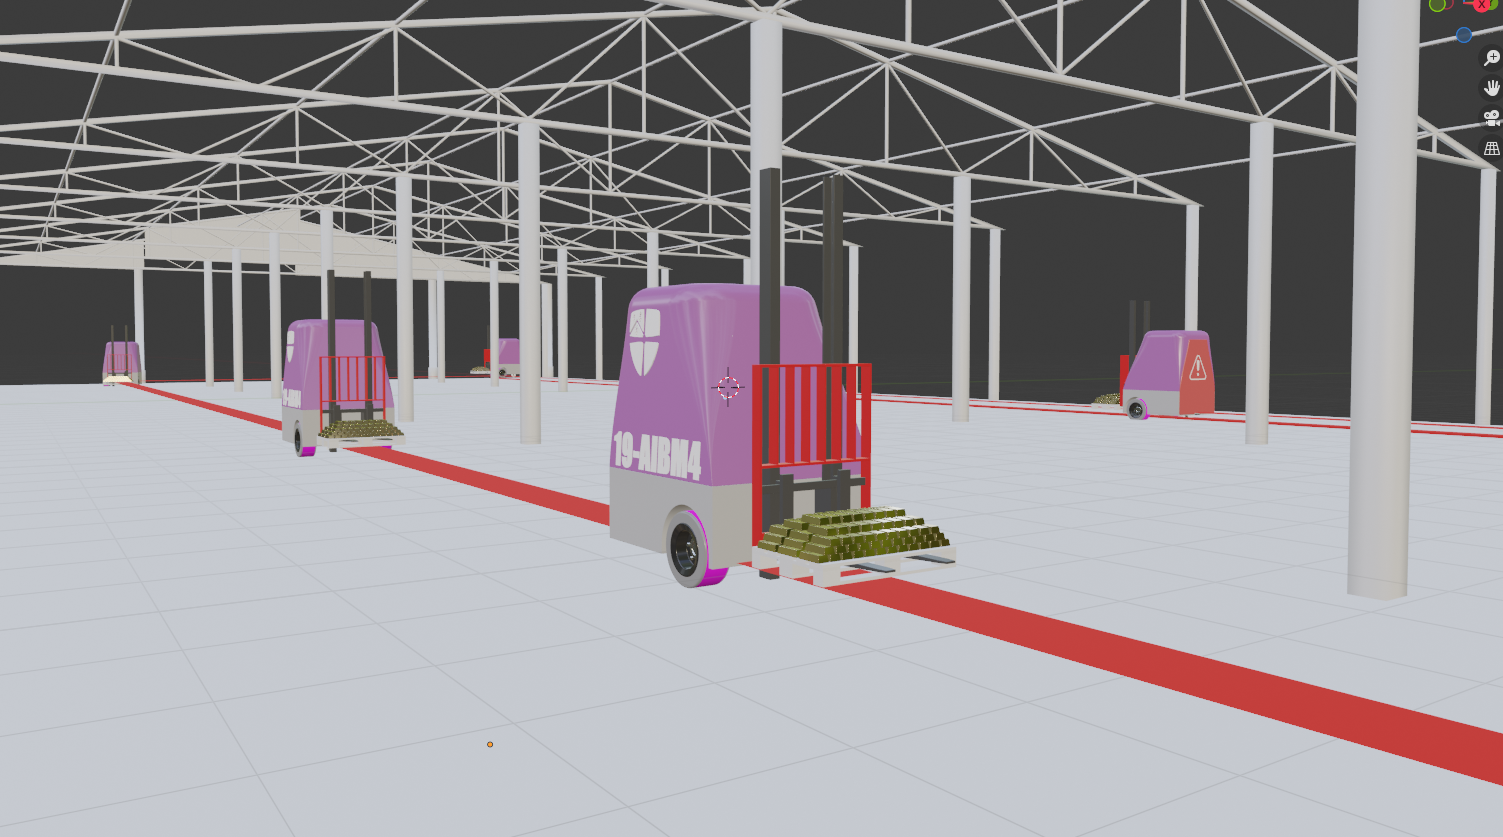
\includegraphics[width=0.5\linewidth]{factory layout1.png}
    \caption{factory design}
    \label{fig:targeted working condition}
\end{figure}
\newpage
\section{User Requirement Specification (URS) for Automated Material Mover (AIBM4)}

\subsection{1. Purpose}
The Automated Material Mover will transport materials effectively, safely, and autonomously within a factory environment. It should reduce manual handling, increase productivity, and ensure a safe working environment.

\subsection{2. Core Requirements}
The Automated Material Mover will:
\begin{itemize}
    \item Operate completely autonomously in predefined zones, performing tasks of moving materials.
    \item Be able to adapt to and cope with various payloads and operational environments.
    \item Include certain safety mechanisms to act safely within its environment.
    \item Have an emergency stop function that can be operated at any time.
    \item Be more efficient than a manual worker and a conventional forklift, i.e., must have a higher uptime.
\end{itemize}

\subsection{3. General Requirements (Should have)}
\begin{itemize}
    \item \textbf{Autonomous Operation:} Capable of navigating, loading, and unloading without any manual intervention.
    \item \textbf{Load Capacity:} Will transport palleted goods of up to 2 tonnes in weight.
    \item \textbf{Environment:} Able to operate in a warehouse setting with smooth and even flooring.
    \item \textbf{Power Supply:} Will operate on rechargeable batteries allowing for a minimum uptime of 8 hours on a single charge, in order to be more efficient than a manual operator.
    \item \textbf{Functional Requirements:} Navigation and obstacle detection, material handling, and speed control.
    \item \textbf{Safety Requirements:} Emergency stop, collision avoidance, and alarm/error detection system.
    \item \textbf{Usability Requirements:} User interface, diagnostics, and maintenance.
    \item \textbf{Environmental Requirements:} Temperature and humidity, and durability.
    \item \textbf{Compliance Requirements:} Safety standards (e.g., ISO 3691-4 on Driverless Industrial Trucks).
    \item \textbf{Reliability:} 99\% uptime over a 1-year period.
    \item \textbf{Error Tolerance:} Less than 1\% failure rate for loading/unloading of goods.
    \item \textbf{Navigation Accuracy:} Reaches the location within 10cm.
\end{itemize}

\subsection{4. Future Enhancements (Could have)}
\begin{itemize}
    \item An advanced obstacle detection and avoidance system.
    \item \textbf{Remote Monitoring and Control:} Potentially over the internet.
    \item \textbf{Dynamic Speed:} Dependent on load and surrounding conditions.
    \item \textbf{Data Logging:} Used to improve performance analysis.
    \item \textbf{Intelligent Task Scheduling:} Algorithm to sort tasks, i.e., machine does tasks near each other in one go.
    \item \textbf{Energy Efficient Mode:} For example, when dealing with light loads.
    \item \textbf{3D Mapping:} Using LiDAR to produce a visualization of the material mover’s current location and route, which can be viewed remotely.
\end{itemize}

\newpage 
 \section{Risk assessment }
 
\begin{figure}[h!]
    \centering
    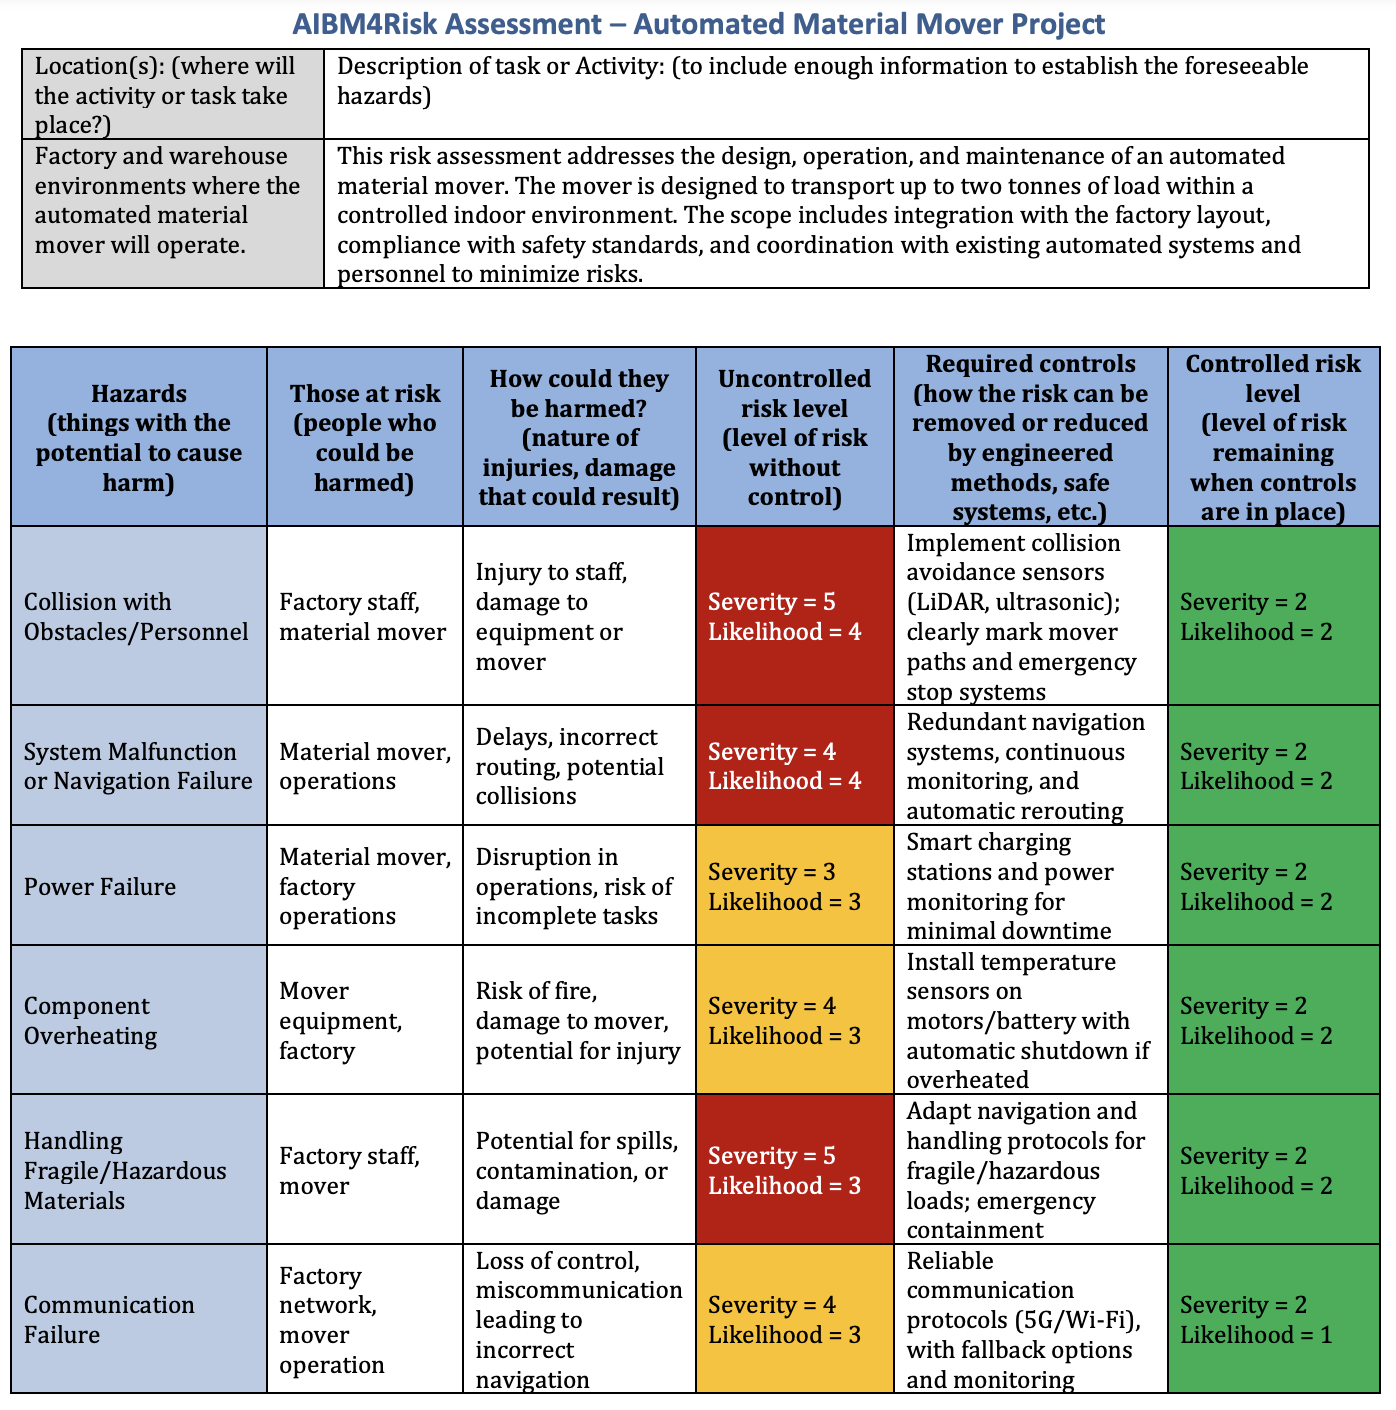
\includegraphics[width=0.9\textwidth]{Risk_Assessment_Automated_Material_Mover_Project1.png}
    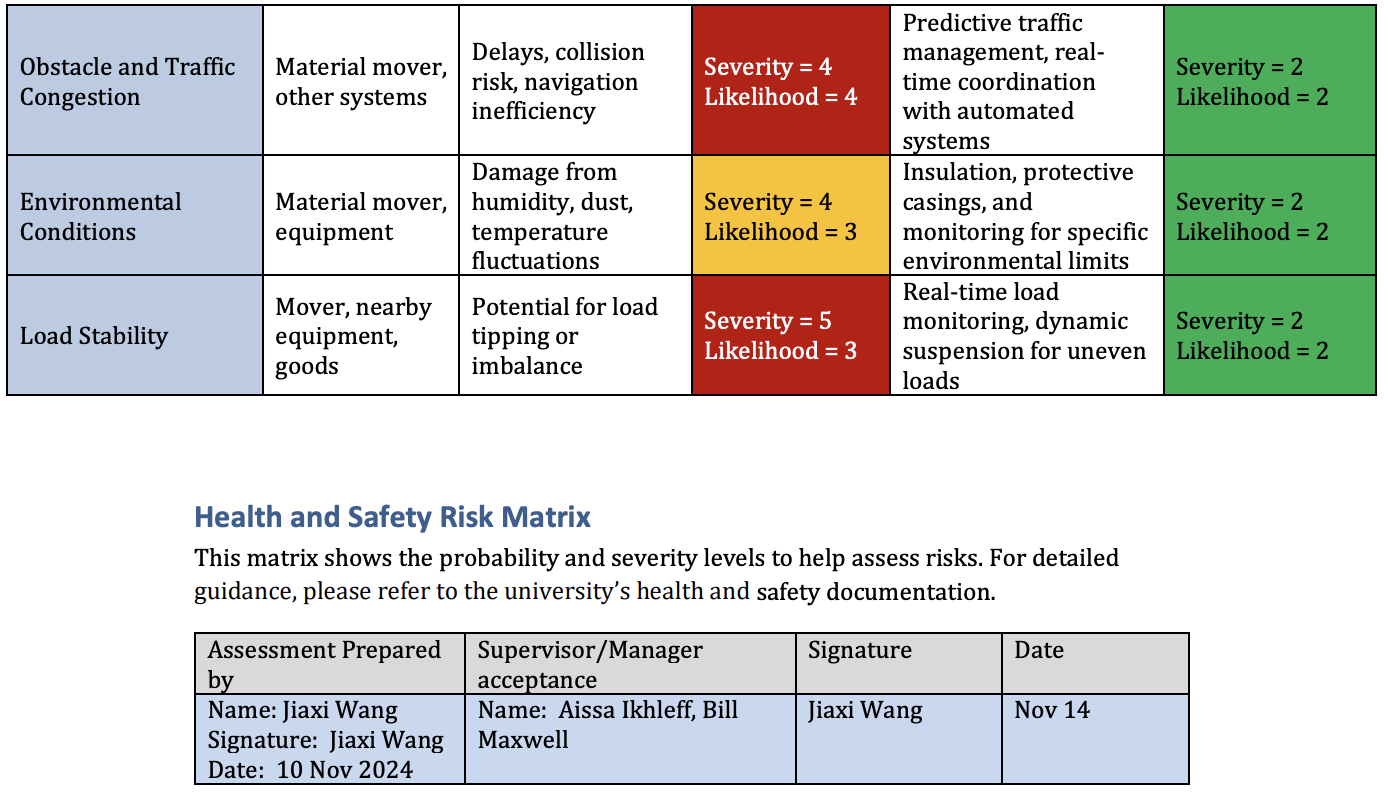
\includegraphics[width=0.9\textwidth]{Risk_Assessment_Automated_Material_Mover_Project2.png}
    \caption{Risk Assessment – Automated Material Mover Project}
    \label{fig:risk_assessment}
\end{figure}



% -------------------------------------------------------------
% 6. Project Schedule
% -------------------------------------------------------------
\section{Project Schedule}

\begin{figure}[h!]
    \centering
    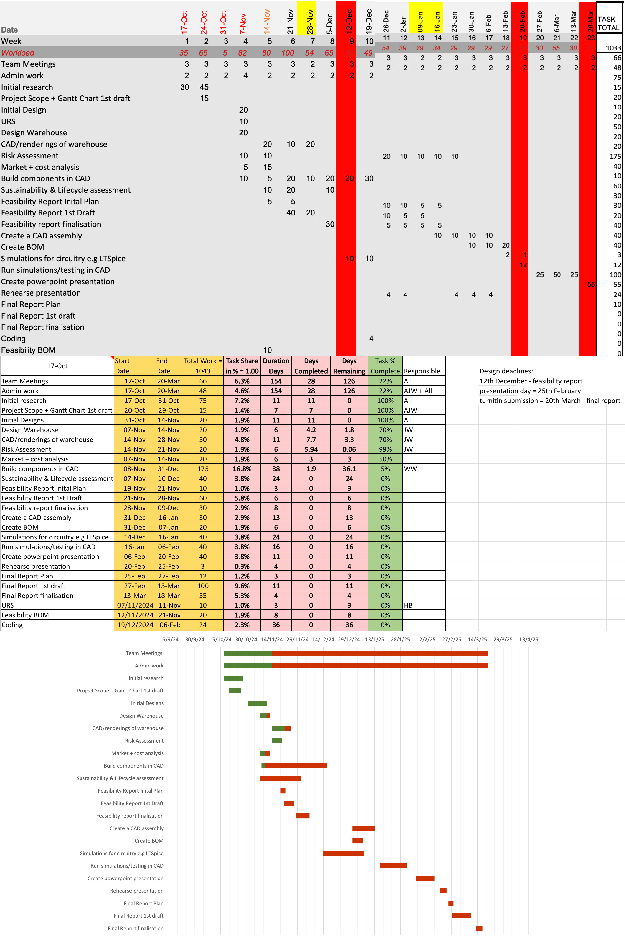
\includegraphics[width=0.9\textwidth]{gantt chart.pdf}
    \caption{Project Gantt Chart}
    \label{fig:timeline}
\end{figure}



% -------------------------------------------------------------
% 7. References
% -------------------------------------------------------------

 \newpage
%\bibliographystyle{unsrt}
%\bibliography{reference}


\begin{thebibliography}{99}

\bibitem{MathWorks}
MathWorks, “What Is SLAM (Simultaneous Localization and Mapping) – MATLAB \& Simulink,” \textit{uk.mathworks.com}.  
Available at: \url{https://uk.mathworks.com/discovery/slam.html} (accessed Nov. 20, 2024).
 

\bibitem{ToyotaForklifts}
Toyota Forklifts, “Automated Warehouse Trucks,” \textit{toyota-forklifts.co.uk}.  
Available at: \url{https://toyota-forklifts.co.uk/automated-solutions/automated-warehouse-trucks/} (accessed Nov. 20, 2024).

\bibitem{Forkify}
Forkify, “Forklift Cost Buyers Guide,” \textit{forkify.com}.  
Available at: \url{https://forkify.com/buyers-guide/forklift-cost/} (accessed Nov. 20, 2024).

\bibitem{LangleyShop}
Langley Shop, “Forklift Forks 100x40x1200 Class 2A,” \textit{langleyshop.co.uk}.  
Available at: \url{https://www.langleyshop.co.uk/product/forklift-forks-100x40x1200-class-2a/} (accessed Nov. 20, 2024).

\bibitem{CheckaTrade}
Checkatrade, “Electric Car Charger Installation Cost,” \textit{checkatrade.com}.  
Available at: \url{https://www.checkatrade.com/blog/cost-guides/electric-car-charger-installation-cost/} (accessed Nov. 20, 2024).

\bibitem{SalaryExpert}
Salary Expert, “Forklift Driver Salary in South Korea,” \textit{salaryexpert.com}.  
Available at: \url{https://www.salaryexpert.com/salary/job/forklift-driver/south-korea?form=MG0AV3} (accessed Nov. 20, 2024).

\bibitem{MordorIntelligence}
Mordor Intelligence, “Automated Material Handling Market,” \textit{mordorintelligence.com}.  
Available at: \url{https://www.mordorintelligence.com/industry-reports/automated-material-handling-market} (accessed Nov. 20, 2024).

\bibitem{GrandViewResearch}
Grand View Research, “Automated Guided Vehicle (AGV) Market,” \textit{grandviewresearch.com}.  
Available at: \url{https://www.grandviewresearch.com/industry-analysis/automated-guided-vehicle-agv-market} (accessed Nov. 20, 2024).

\end{thebibliography}


 

% -------------------------------------------------------------

% -------------------------------------------------------------
% BIBLIOGRAPHY (LOCAL) - Uncomment to use instead of BIB
% -------------------------------------------------------------
% \thebibliography{file}
% \begin{thebibliography}{99}                                   % Start bibliography
% %                                                             % Can be in a separate file, \input(...)
% \bibitem{Bonfanti:2016ab} A. Bonfanti, A. Bhaskar, M.F. Ashby.                      % Author names
%         Plastic deformation of cellular materials,                                  % Title of publication
%         \textit{Reference Module in Materials Science and Materials Engineering},   % Journal name
%         2016.                                                                       % Vol, num, pg, year
% %
% \bibitem{Lee:2017aa} J.H. Lee, D.R. Howel, W.P. Meehan III, G.L. Iverson, A.J. Gardner.
%         Effects of Exercise on Sport Concussion Assessment Tool--Third Edition Performance in Professional Athletes,
%         \textit{The Orthopaedic Journal of Sports Medicine},
%         \textbf{5}(9):1--7, 2017. 
% %
% \bibitem{Lang:1988aa} R.J. Lang.
%         \textit{The complete book of origami: Step-by-step instructions in over 1000 diagrams},
%         Dover Publications, Inc.
%         1988. 
% %
% \bibitem{Kingslake:1992aa} R. Kingslake.
%         \textit{Optics in photography},
%         SPIE Optical engineering press
%         1992. 
% %
% \bibitem{Chen:2011ab} W. Chen, B. Song.
%         \textit{Split Hopkinson (Kolsky) bar: Design, Testing and Applications},
%         Mechanical Engineering Series, Springer
%         2011. 
% %
% \bibitem{Fairlie:2008aa} G.E. Fairlie, R. Hart, E.J. Draper.
%         \textit{Structural response to high explosive blast loading},
%         in MABS 20 - Military Aspects of Blast and Shock,
%         2008. 
% %
% \end{thebibliography}                                         % End bibliography

% -------------------------------------------------------------
% LISTS OF FIGURES AND TABLES
% -------------------------------------------------------------
\listoffigures                                                % Add list of figures
\listoftables                                                 % Add list of tables

% -------------------------------------------------------------
% WORD COUNT OUTPUT


% 8. Appendices
% -------------------------------------------------------------
\section{Appendices}
Additional charts, data, or images can be included here.

\end{document}
